\documentclass[12pt]{article}
\usepackage{geometry}                % See geometry.pdf to learn the layout options. There are lots.
\geometry{letterpaper}                   % ... or a4paper or a5paper or ... 
%\geometry{landscape}                % Activate for for rotated page geometry
\usepackage[parfill]{parskip}    % Activate to begin paragraphs with an empty line rather than an indent
\usepackage{daves,fancyhdr,natbib,graphicx,dcolumn,amsmath,lastpage,url}
\usepackage{amsmath,amssymb,epstopdf,longtable}
\usepackage{paralist}  % need to properly formulate standard answer blocks
\usepackage[final]{pdfpages}
\DeclareGraphicsRule{.tif}{png}{.png}{`convert #1 `dirname #1`/`basename #1 .tif`.png}
\pagestyle{fancy}
\lhead{CE 3305 Fluid Mechanics; Exercise Set 10}
\rhead{Name:\_\_\_\_\_\_\_\_\_\_\_\_\_\_\_\_\_\_\_\_\_\_\_\_\_\_\_\_\_\_\_\_\_\_}
\lfoot{REVISION A}
\cfoot{}
\rfoot{Page \thepage\ of \pageref{LastPage}}
\renewcommand\headrulewidth{0pt}
%%%%%%%%%%%%%%%%%%%%%%%%%%%%%%%%%%%%
\begin{document}
%%%%%%%%%%%%%%%%%%%%%%%%%%%%%%%%%%%
\begingroup
\begin{center}
{\textbf{{ CE 3305 Engineering Fluid Mechanics} \\ Exercise Set 10 \\ Summer 2018 -- GERMANY} }
\end{center}
\endgroup
\begingroup
~\newline
\textbf{Purpose} :  Application of continunity to relate flow area and velocity to volumetric (or mass) flow rate. \\
\textbf{Assessment Criteria} : Completion, plausible solutions, use \textbf{R} as a calculator. \\~\\
\textbf{Exercises}

\begin{enumerate}
\item (Problem 5.9 pg 196)  A pipe with a 2 $m$ diameter carries water with mean section velocity of 4 $m/s$.  What is the volumetric discharge in cubic meters per second?

\item (Problem 5.20 pg 197) Figure \ref{fig:OpenChannel} is a schematic of flow in a rectangular channel that is 1.2 $m$ wide.   The velocity distribution measured perpendicular from the channel bottom is shown on the figure.  Estimate the discharge in the channel.

\begin{figure}[h!] %  figure placement: here, top, bottom, or page
   \centering
   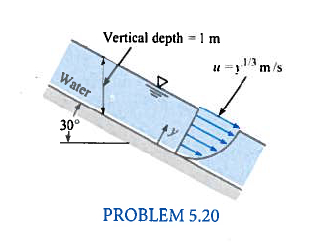
\includegraphics[width=3.5in]{OpenChannel.jpg} 
   \caption{Velocity distribution in a rectangular channel.}
   \label{fig:OpenChannel}
\end{figure}

\item (Problem 5.23 pg 197) Water enters the lock of a ship canal through 180 ports, each port having a 2 $ft$ (0.6 $m$) by 2 $ft$ (0.6 $m$) cross section.  The lock is 900 $ft$ (274.4 $m$ ) long and 105 $ft$ (32.01 $m$ ) wide.
The lock is designed so that the water surface in it will rise at a maximum rate of 6 $ft/min$ (1.83 $m/min$).   For this condition, what is the mean section velocity in each port?

\end{enumerate}


\end{document}  